\documentclass[a4paper, 11pt]{report}

%%%%%%%%%%%%
% Packages %
%%%%%%%%%%%%

\usepackage[english]{babel}
\usepackage{packages/sleek}
\usepackage{packages/sleek-title}
\usepackage{packages/sleek-theorems}
\usepackage{packages/sleek-listings}
\usepackage{import}

%%%%%%%%%%%%%%
% Title-page %
%%%%%%%%%%%%%%

%\logo{./resources/pdf/logo.pdf}
\institute{Kybernetika a umělá inteligence}
\faculty{B3B33KUI}
%\department{Department of Anything but Psychology}
\title{Výber klasifikátoru}
% \subtitle{Distributed embedded data acquisition system of an experimental rocket}
\author{Ondrej Nečas}
%\supervisor{Linus \textsc{Torvalds}}
\context{Template: \href{https://github.com/francois-rozet/sleek-template.git}{github.com francois-rozet sleek-template}}
\date{\today}

%%%%%%%%%%%%%%%%
% Bibliography %
%%%%%%%%%%%%%%%%

%\addbibresource{./resources/bib/references.bib}

%%%%%%%%%%
% Macros %
%%%%%%%%%%

\newcommand{\tbs}{\textbackslash}

%%%%%%%%%%%%
% Document %
%%%%%%%%%%%%

\begin{document}
    \maketitle
%    \newpage
%    \pagenumbering{roman}
%    \tableofcontents
    \newpage
    \pagenumbering{arabic}

    \section*{1. Výber vhodného parametru}\label{sec:parameter-selection}

    Pre klasifikátor 1 \textbf{(C1.dsv)} sú najlepšie parametry $\alpha$ medzi 8 až 24.

    \begin{wrapfigure}{r}{0.5\textwidth} % "r" for right alignment, "0.5\textwidth" for the width of the figure
        \centering
        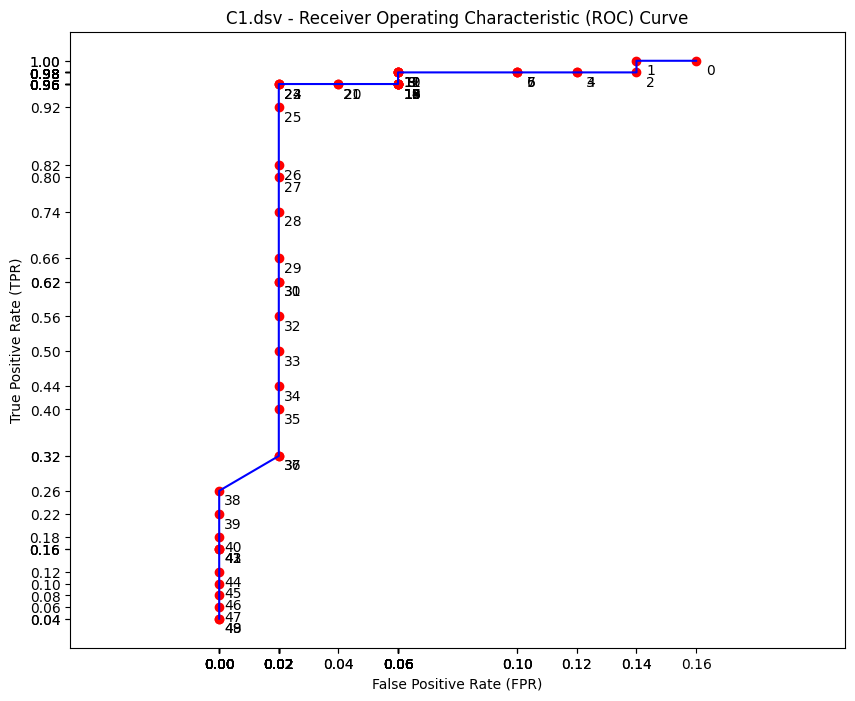
\includegraphics[width=0.6\textwidth]{images/first} % slightly less than wrapfigure width to fit properly
%    \caption{C1 ROC}
        \label{fig:c1-roc}
    \end{wrapfigure}

    Pre generický binárny klasifikátor (True/Flase) predpokladáme, že vyžadujeme vysokú mieru senzitivity (správne identifikované
    True prípady). Rozumný kompromis medzi TPR (True Positive Rate) a FPR (False Positive Rate), pri ktorom uprednostňujeme TPR. Tá by mala byť
    čo najvyššia, aby sme zabezpečili vysokú úspešnosť klasifikácie daného objektu TP (True Positives) s nízkym zastúpením FP (False Positives).

    Pre každý paramter $\alpha$ (0..49) vypočítame TPR, FPR. Po zobrazení sú najlepšie parametre v rozmedzí 8 až 24, nakoľko majú
    vysoký podiel klasifikácií skutočných 'True' objektov na 'True' (nad 90\% zo všetkých 'True' klasifikácií) a relatívne
    nízky podiel klasifikácie skutočných 'False' objektov na 'True' (pod 6\% zo všetkých skutočných 'False' objektov).

    \section*{2. Prísne tajné!}\label{sec:top-secret}

    Klasifikátor 4 \textbf{(C4.dsv)} s $\alpha$ 11.

    \begin{wrapfigure}{r}{0.5\textwidth} % "r" for right alignment, "0.5\textwidth" for the width of the figure
        \centering
        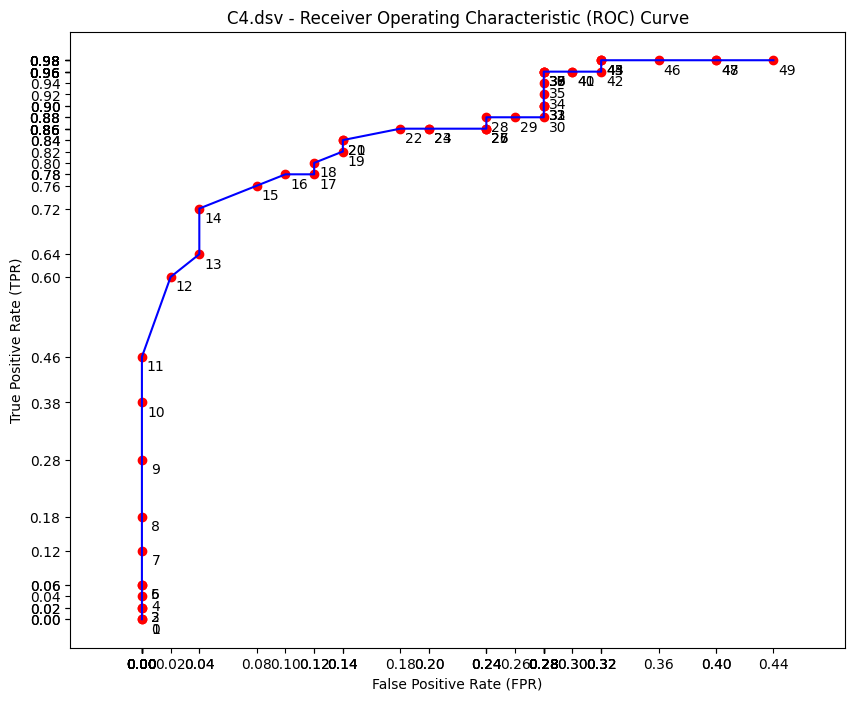
\includegraphics[width=0.6\textwidth]{images/second} % slightly less than wrapfigure width to fit properly
%    \caption{C1 ROC}
        \label{fig:c2-roc}
    \end{wrapfigure}

    Pri zabezpečení tajných dokumentov vyžadujeme vysokú specifitu (správne identifikované False prípady). Uprednostníme
    nízku mieru FPR, aby sme sa vyhli nežiadúcemu prístupu k tajným informáciam prostredníctvom FP. Následne budeme
    hodnotiť na základe najvyššej TPR. Pripúšťame mať vyššie FN (False negatives) nad povolením akýchkoľvek FP (False positives).

    Klasifikátor 4 s $\alpha$ 11 má mieru FPR (0\%) a spomedzi ostatných klasifikátorov najvyššiu mieru TPR (46\%).
    Čiže by určite nepripustil nikoho, kto by sa pokúsil získať prístup k týmto dokumentom a nemal by. Samozrejme,
    vychádzame z testovacích dát.

    \section*{3. Hlavne bezpečne}\label{sec:mainly-securely}

    Moja funkcia bude pracovať s úvahou ako v minulej sekcii. Rozhoduje na základe najnižšieho FPR, a následne najvyššieho TPR z dostupných klasifikátorov.
    Ak bude mať nový klasifikáto FPR rovnú 0\% a vyššiu TPR ako 46\% , tak bude vybraný ako nový klasifikátor. Za predpokladu, že
    budeme pracovať na rovnakých trénovacích dátach ako doteraz.

\end{document}
